%%%%%%%%%%%%%%%%%%%%%%%%%%%%%%%%%%%%%%

%\usepackage[scale=0.8,size=a1]{beamerposter} and using \setlength{\paperwidth}{36in} and \setlength{\paperheight}{24in}

\documentclass[final]{beamer}
\usepackage[scale=0.8,size=a1]{beamerposter}
\usepackage{graphicx,bm,color}
\usepackage{tikz}
\usepackage{tcolorbox}
\definecolor{darkblue}{rgb}{0.0,0.0,0.50}
\definecolor{myorange}{rgb}{1.0,0.4,0.0}
\newcommand{\highlt}{\textcolor {myorange}}
\newcommand{\citeme}{\textcolor {blue}}


%-----------------------------------------------------------
% Define the column width and poster size
% To set effective sepwid, onecolwid and twocolwid values, first choose how many columns you want and how much separation you want between columns
% The separation I chose is 0.024 and I want 4 columns
% Then set onecolwid to be (1-(4+1)*0.024)/4 = 0.22
% Set twocolwid to be 2*onecolwid + sepwid = 0.464
%-----------------------------------------------------------

\newlength{\sepwid}
\newlength{\onecolwid}
\newlength{\twocolwid}
\newlength{\threecolwid}
\setlength{\paperwidth}{36in}
\setlength{\paperheight}{24in}
\setlength{\sepwid}{0.024\paperwidth}
\setlength{\onecolwid}{0.22\paperwidth}
\setlength{\twocolwid}{0.464\paperwidth}
\setlength{\threecolwid}{0.708\paperwidth}
\setlength{\topmargin}{-0.5in}
\usetheme{confposter}
\usepackage{exscale}

\usecaptiontemplate{
\small
\structure{\insertcaptionname~\insertcaptionnumber:}
\insertcaption}


%-----------------------------------------------------------
% Define colours (see beamerthemeconfposter.sty to change these colour definitions)
%-----------------------------------------------------------

\setbeamercolor{block title}{fg=myorange,bg=white}
\setbeamercolor{block body}{fg=black,bg=white}
\setbeamercolor{block alerted title}{fg=white,bg=darkblue!70}
\setbeamercolor{block alerted body}{fg=black,bg=dblue!10}

%-----------------------------------------------------------
% Name and authors of poster/paper/research
%-----------------------------------------------------------

\title{\large Exploring the role of gene interaction in idiopathic pulmonary fibrosis with exome sequencing \normalsize}
\author{\normalsize Adam J Richards$^{1}$, Tasha Fingerlin$^{2}$, Ivana V. Yang$^{1}$, James E. Loyd$^{3}$, Debbie A. Nickerson$^{4}$, Elizabeth Blue$^{4}$, Karynne Patterson$^{4}$, and David A. Schwartz$^{1}$}
\institute{\small $^{1}$University of Colorado Denver, CO, USA \\ 
$^{2}$Colorado School of Public Health, CO, USA \\
$^{3}$Vanderbilt University, TN, USA \\
$^{4}$University of Washington, WA, USA \normalsize
}

%-----------------------------------------------------------
% Start the poster itself
%-----------------------------------------------------------
% The \rmfamily command is used frequently throughout the poster to force a serif font to be used for the body text
% Serif font is better for small text, sans-serif font is better for headers (for readability reasons)
%-----------------------------------------------------------

\begin{document}
\addtobeamertemplate{headline}{} 
% {\begin{tikzpicture}[remember picture, overlay]
%      \node [anchor=north east, inner sep=3cm]  at (current page.north east)
%      {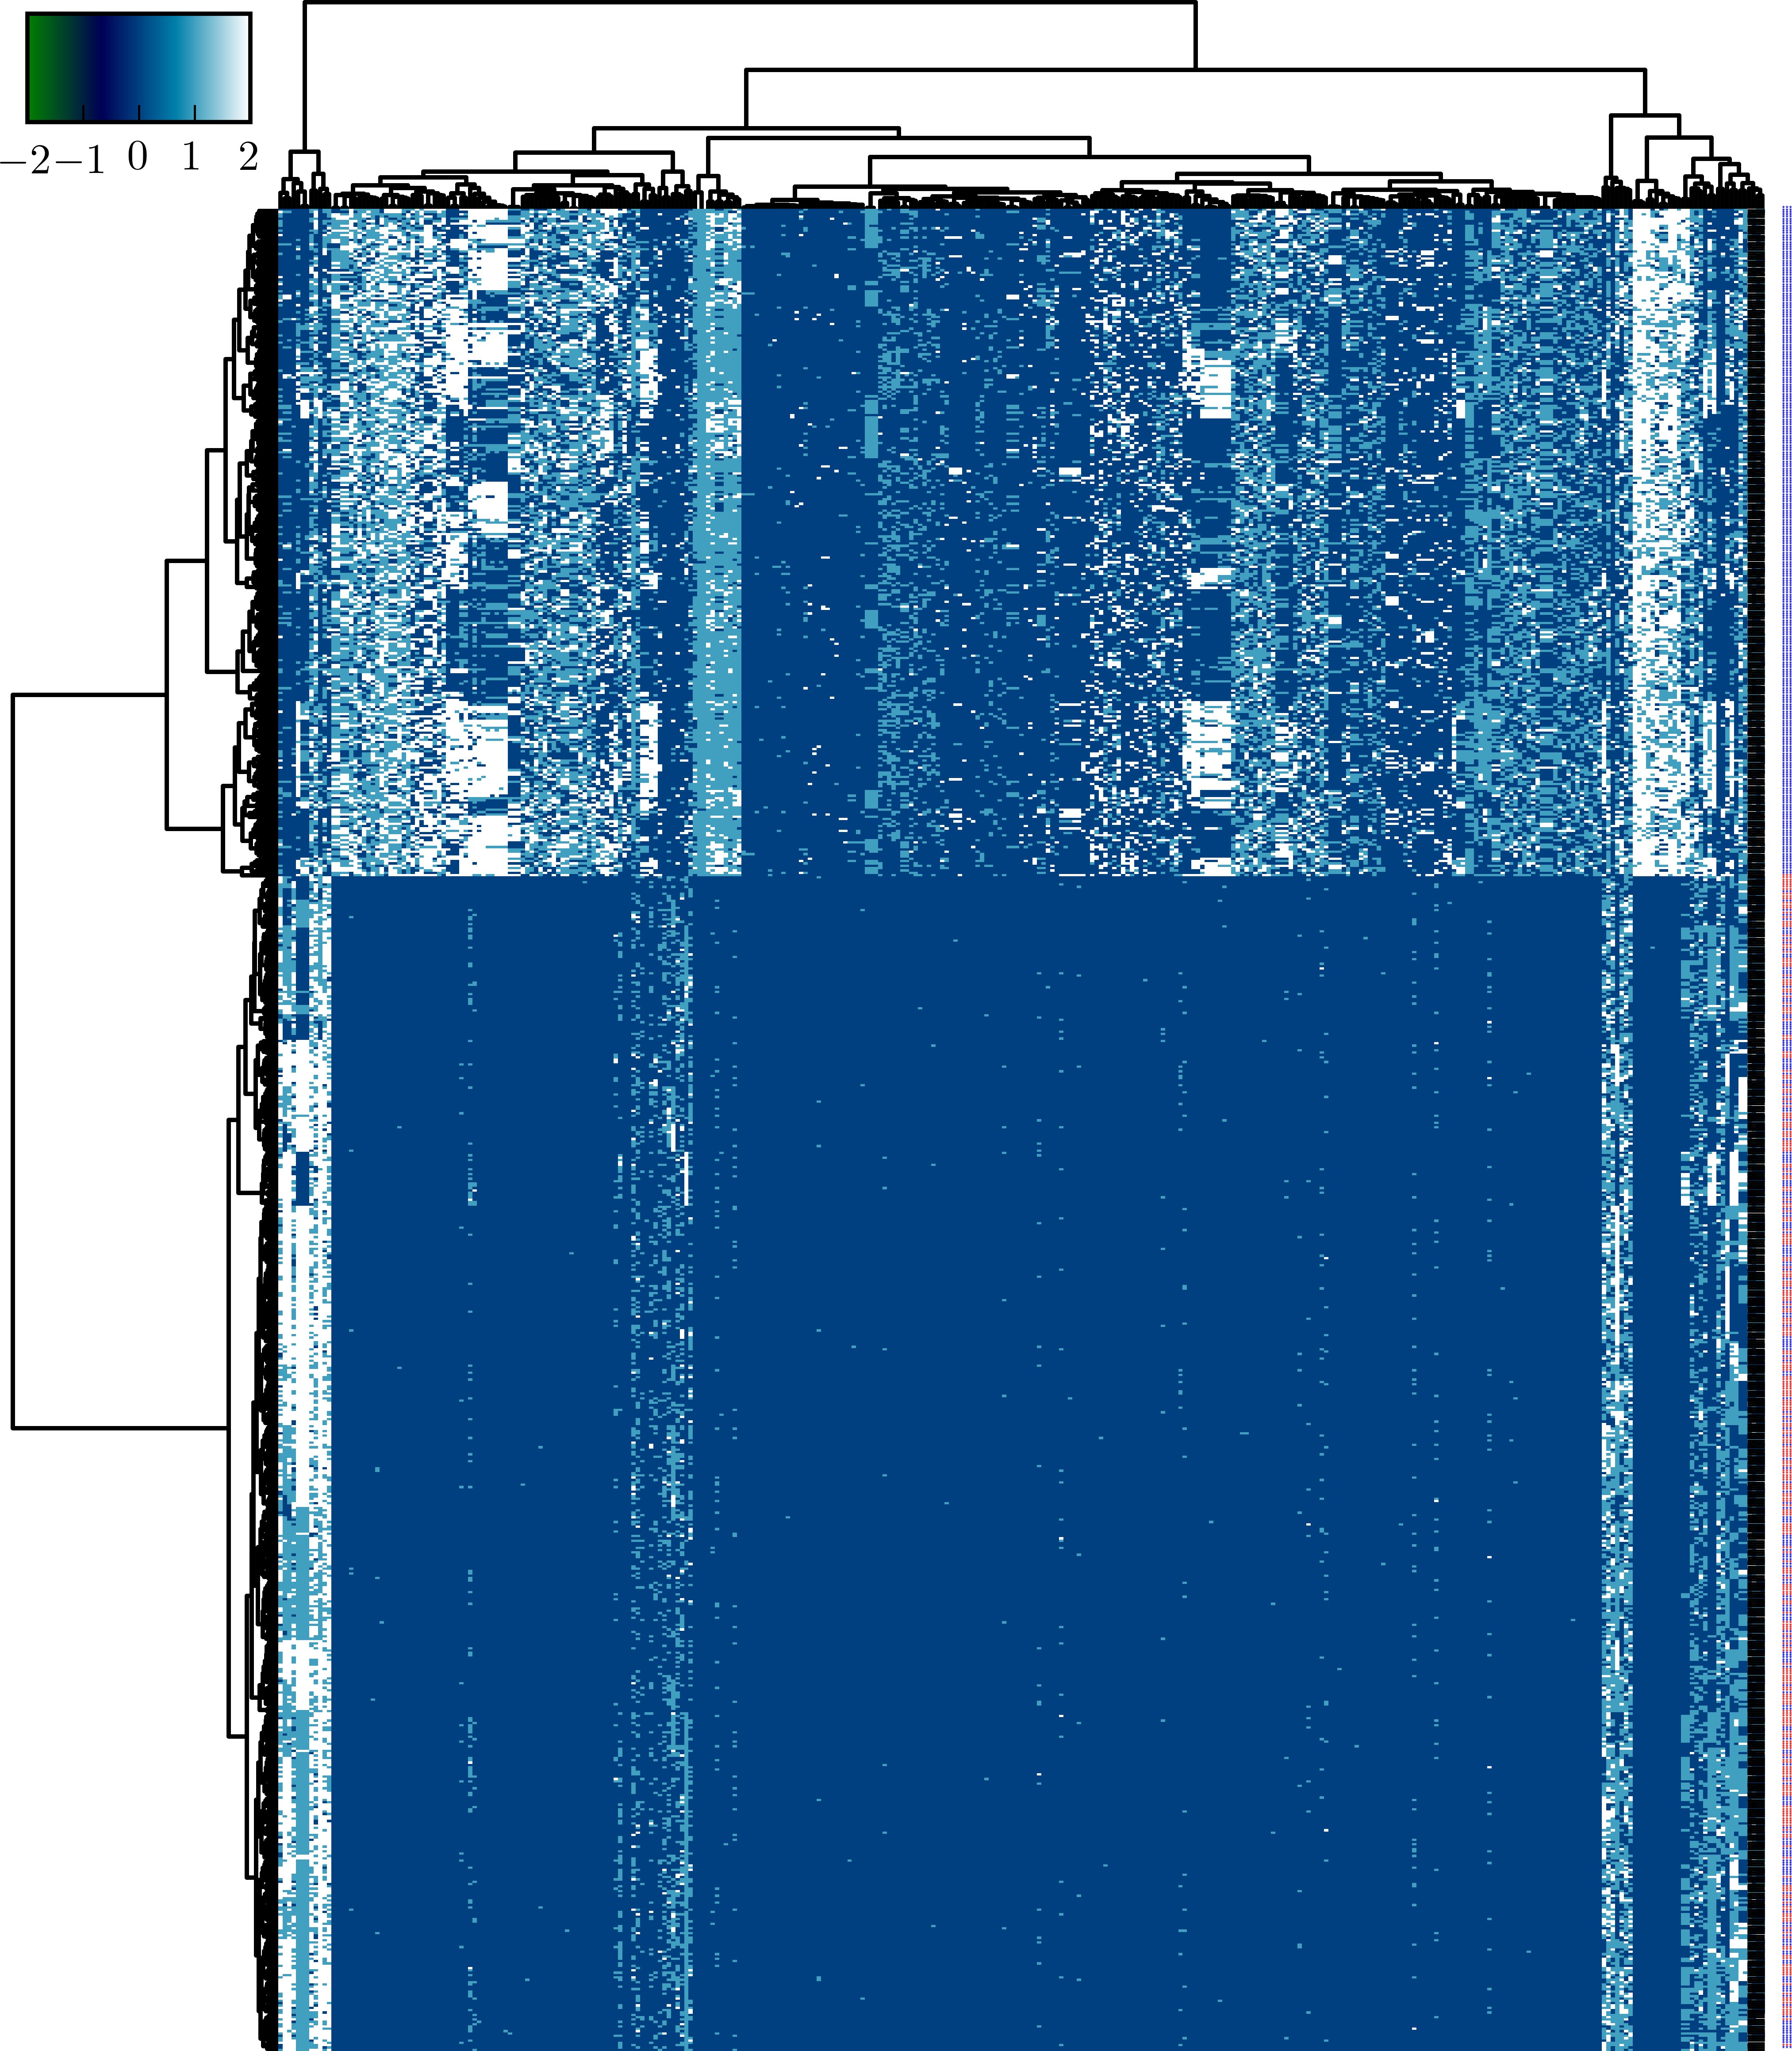
\includegraphics[height=6cm]{./figs/clustered-heatmap-all.png}};
%   \end{tikzpicture}}

\addtobeamertemplate{headline}{}   
 {\begin{tikzpicture}[remember picture, overlay]
      \node [anchor=north west, inner sep=3cm]  at (current page.north west)
      {\includegraphics[height=3cm]{./figs/cu-anschutz.jpg}};
   \end{tikzpicture}}
  
\begin{frame}[t]
\begin{columns}[t] % the [t] option aligns the column's content at the top
    \begin{column}{\sepwid}\end{column}
    \begin{column}{\onecolwid}
      \begin{block}{Deep Quality Networks}
      \small
    \rmfamily{Deep-Q Networks apply reinforcement learning to neural networks. The network predicts Q-values for each action the network is allowed. A Q-value represents quality of a state, or the expected sum of rewards as we play the game from that state. Our agents (almost) always select the max Q-value we predict. DQN's were deployed to great effect by DeepMind, most recently in their Go-playing AI, AlphaGo.}
      \end{block}
      \begin{block}{Background}
        \rmfamily{\small
      \begin{itemize}\justifying
          \item \textbf{\highlt{Goal 1: Simulation}} demonstrating DQN's
          \item \textbf{\highlt{Goal 2: Physical deployment}} of a DQN to control a Sphero
          \item \textbf{\highlt{Goal 3: Navigation}} through a complex space using DQN
      \end{itemize}
      }
      \end{block}
       \begin{block}{Approach}
       \rmfamily{\small
        \begin{itemize}\justifying
          \item 286 cases
          \item variant association based on frequency differences
          \item variant interaction inferred by an iterative support vector machines approach
        \end{itemize}
       }
       \end{block}
       \begin{block}{Variant calling}
        \rmfamily{\small
        \begin{figure}
            \begin{center}
              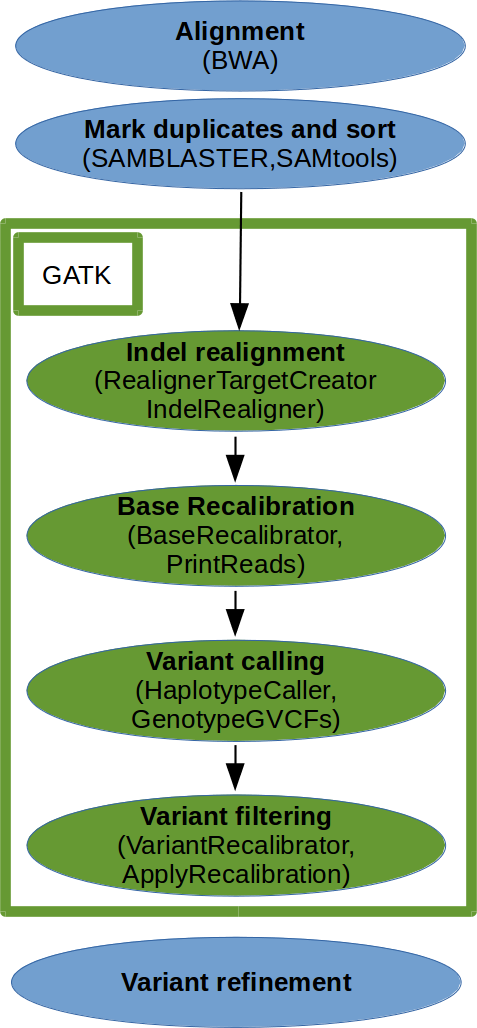
\includegraphics[width=3in]{./figs/pipeline.png}
            \end{center}
            \caption{Variant calling pipeline based on BWA \cite{Li09} and GATK \cite{McKenna10}}
            \label{fig:pipeline} 
            \end{figure}
           }
    \end{block}
   \end{column}
    %%%%%%%%%%%%%%%%%%%%%%%%%%%%%%%%%%%%%%%%%%%%%%%%%%%%%%%%%%%%%%%%%%%%%%%%%%%%%%%%%%%%%%%%%%%%%%%%%%%%%%%%%%%%%
    % column 2
    %%%%%%%%%%%%%%%%%%%%%%%%%%%%%%%%%%%%%%%%%%%%%%%%%%%%%%%%%%%%%%%%%%%%%%%%%%%%%%%%%%%%%%%%%%%%%%%%%%%%%%%%%%%%%
    \begin{column}{\sepwid}\end{column}
    \begin{column}{\onecolwid}
    \begin{block}{Variant association}
       \small
       \rmfamily{
       For each variant we subtract the case major allele frequency from the G1K reference population (EUR) to obtain frequency distributions.
       \begin{figure}
           \begin{center}
             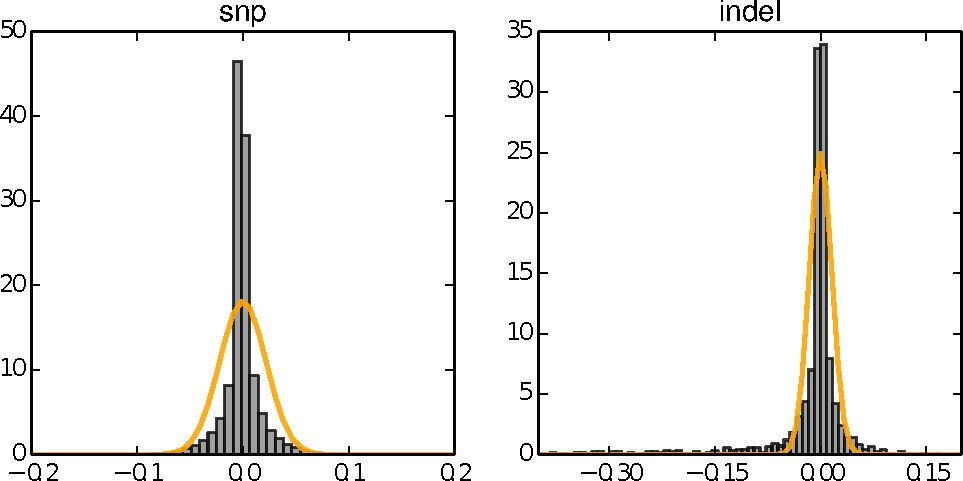
\includegraphics[width=6in]{./figs/raw-frq-diffs.pdf}
           \end{center}
           \begin{flushleft}\small{\color{darkblue}Figure 1: \color{black} Frequency differences between called variants in the case cohort and variants in the G1K reference data.  }\end{flushleft}.
           \label{fig:frq-diffs} 
           \end{figure}
          }
        \rmfamily{
	 The null hypothesis is that there is no difference in major allele frequency between the cases and controls. the frequency difference distributions were fit with Gaussians.  The skewed indel distribution was fit by ignoring the tails.  To test the significance of the $i$th frequency difference $f$ we simply use a two-sided $Z$-test.
	\begin{equation}
	 z_{i} = \frac{f_{i}}{\sigma}
	\end{equation}
        $p$-values were then obtained according to $2\Phi(-|z_{i}|)$, where $\Phi$ is the normal CDF.  We controlled for multiple testing using the Benjamini and Hochberg FDR method \cite{Benjamini95}.
       \begin{figure}
           \begin{center}
             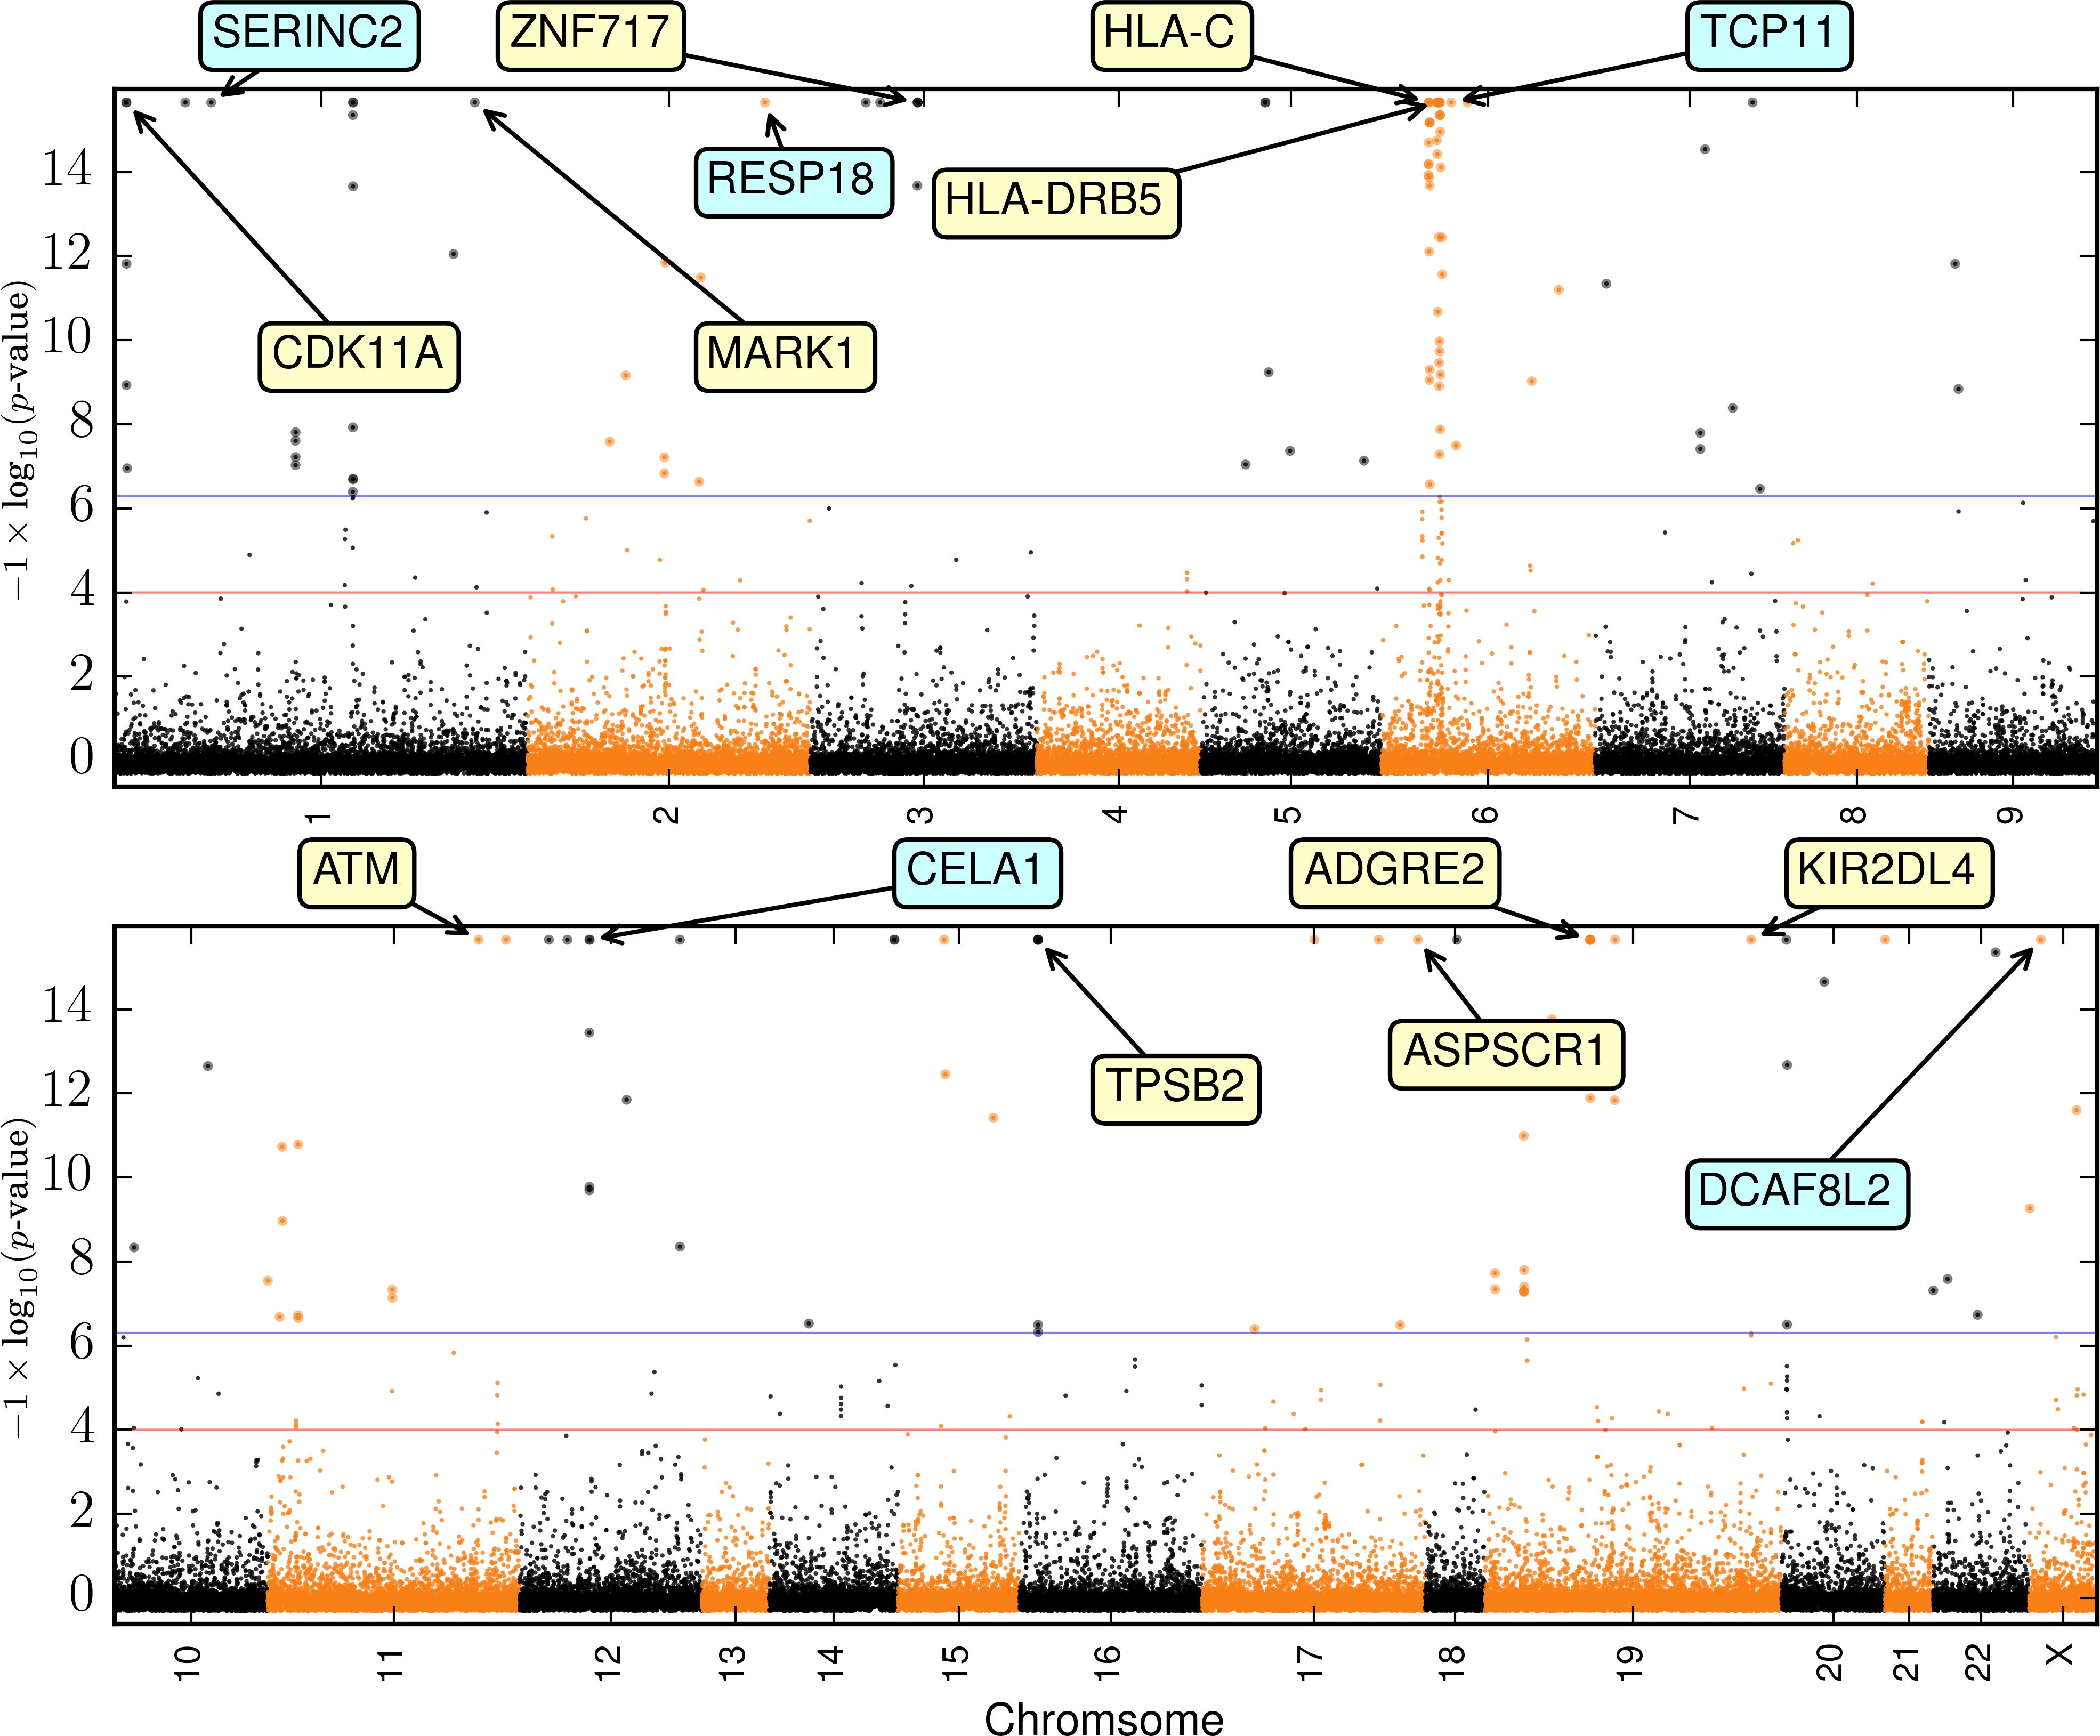
\includegraphics[width=7in]{./figs/manhattan-diffs.png}
           \end{center}
           \begin{flushleft}\small{\color{darkblue}Figure 3: \color{black} Manhattan plot of the $p$-values based on frequency differences.  The top 15 variants are shown with the light oranges and blues indicating SNP and indels respectively.  The two drawn thresholds correspond to $0.001$ and $5*10e-08$.}\end{flushleft}.
           \label{fig:manhattan} 
           \end{figure}
           \begin{tcolorbox}
           Variants from the HLA region were were highly associated with disease along with several Mucin genes (MUC2, MUC6, and MUC16)
          \end{tcolorbox} 
          }
           \end{block}
    \end{column}
    
    %%%%%%%%%%%%%%%%%%%%%%%%%%%%%%%%%%%%%%%%%%%%%%%%%%%%%%%%%%%%%%%%%%%%%%%%%%%%%%%%%%%%%%%%%%%%%%%%%%%%%%%%%%%%%
    % Third column
    %%%%%%%%%%%%%%%%%%%%%%%%%%%%%%%%%%%%%%%%%%%%%%%%%%%%%%%%%%%%%%%%%%%%%%%%%%%%%%%%%%%%%%%%%%%%%%%%%%%%%%%%%%%%%
    \begin{column}{\sepwid}\end{column}
    \begin{column}{\onecolwid}
       \begin{block}{Gene-Gene interaction}
       \small
       \rmfamily{
	\begin{table}
	\begin{center}
       \begin{tabular}{l|c|c|c}
       \hline
       variant  & $0.001$ & $5*10e-08$ & B-H adjusted \\
       \hline
       SNP      & 413        & 142        & 274\\
       indel    & 59         & 27         & 63 \\ 
       \end{tabular}
       \end{center} 
       \begin{flushleft}\small{\color{darkblue}Table 1: \color{black} Summary of candidate variants.}\end{flushleft}.
           \label{fig:manhattan}
       \end{table}
       }  
       \rmfamily{
       Imputed genotypes for both the cases and controls were transformed into $\{0,1,2\}$ space which represents reference, heterozygous-alternative and homozygous-alternative respectively.
        \begin{figure}
            \begin{center}
              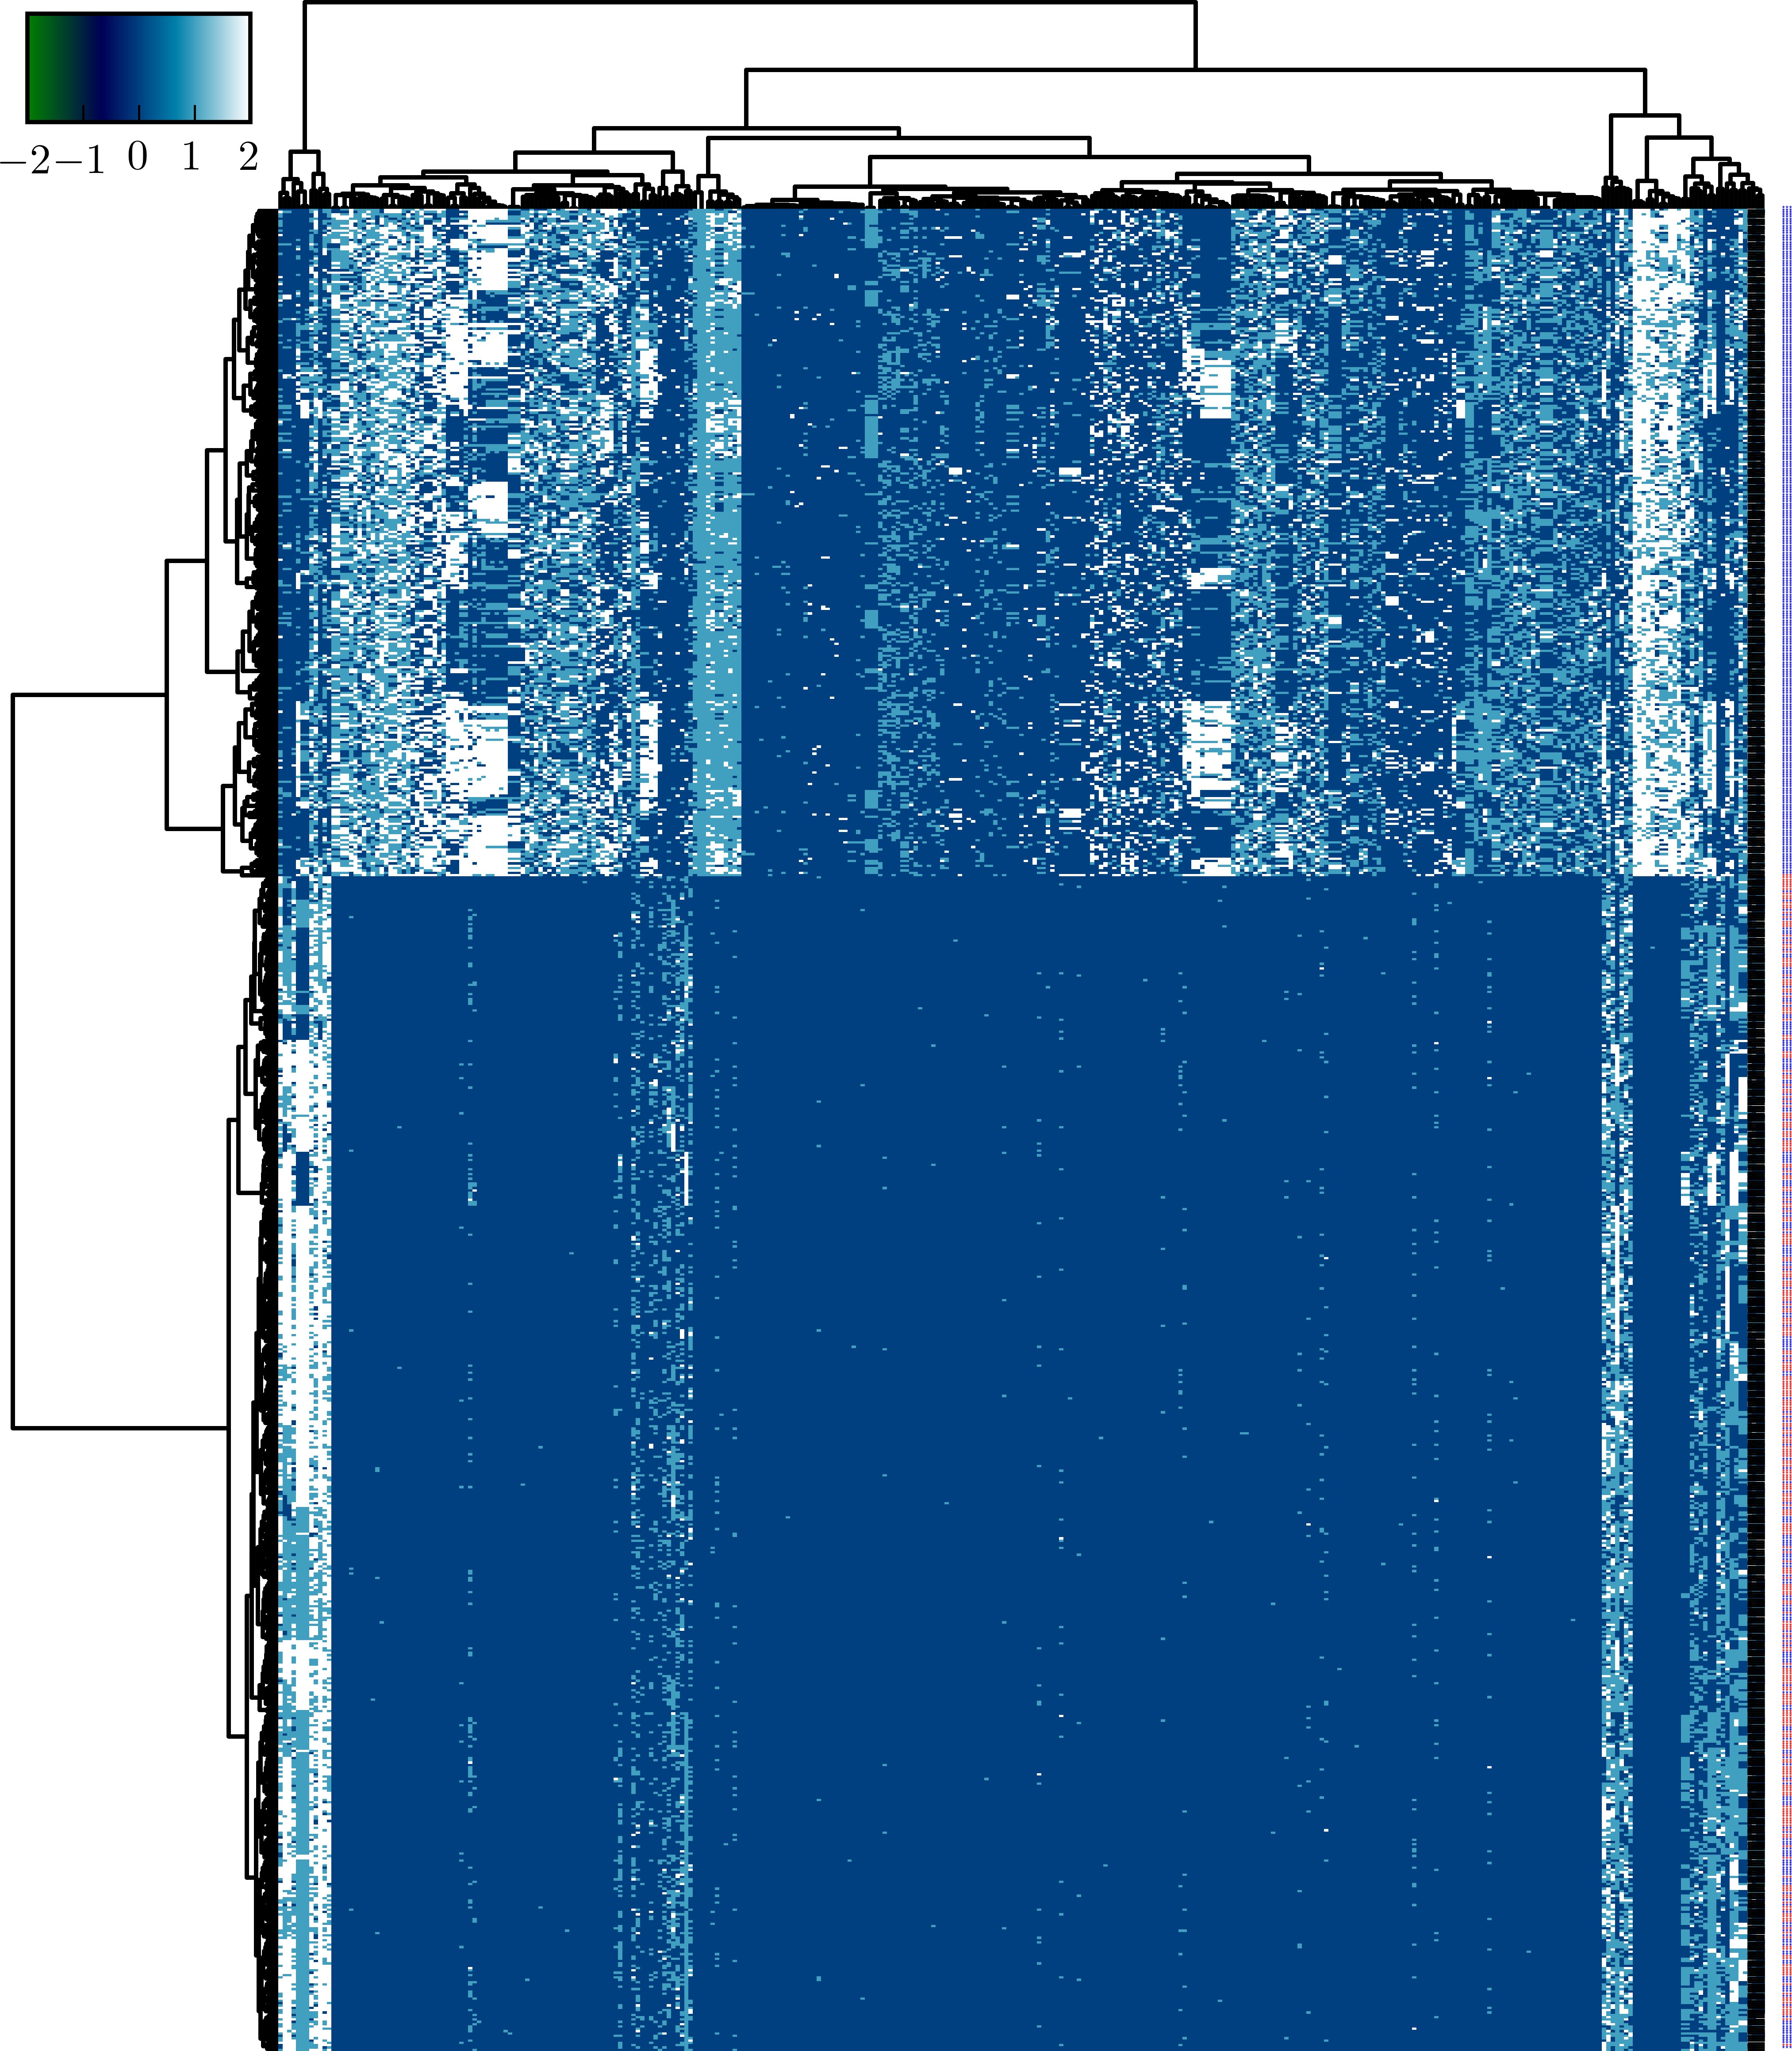
\includegraphics[width=4.5in]{./figs/clustered-heatmap-all.png}
            \end{center}
            \begin{flushleft}\small{\color{darkblue}Figure 4: \color{black} Imputed genotypes were discretized for input into machine learning algorithms.  Here the values are shown with a clustering at the sample level (rows) and variant level (columns)  The cases and reference population are readily distinguishable.
            }\end{flushleft}.
            \label{fig:heatmap} 
            \end{figure} 
            
	Of the 337 variants with significant $p$-values after adjustment we only considered the 279 with minor allele frequencies $\geq$ 5\%.
        \begin{figure}
            \begin{center}
              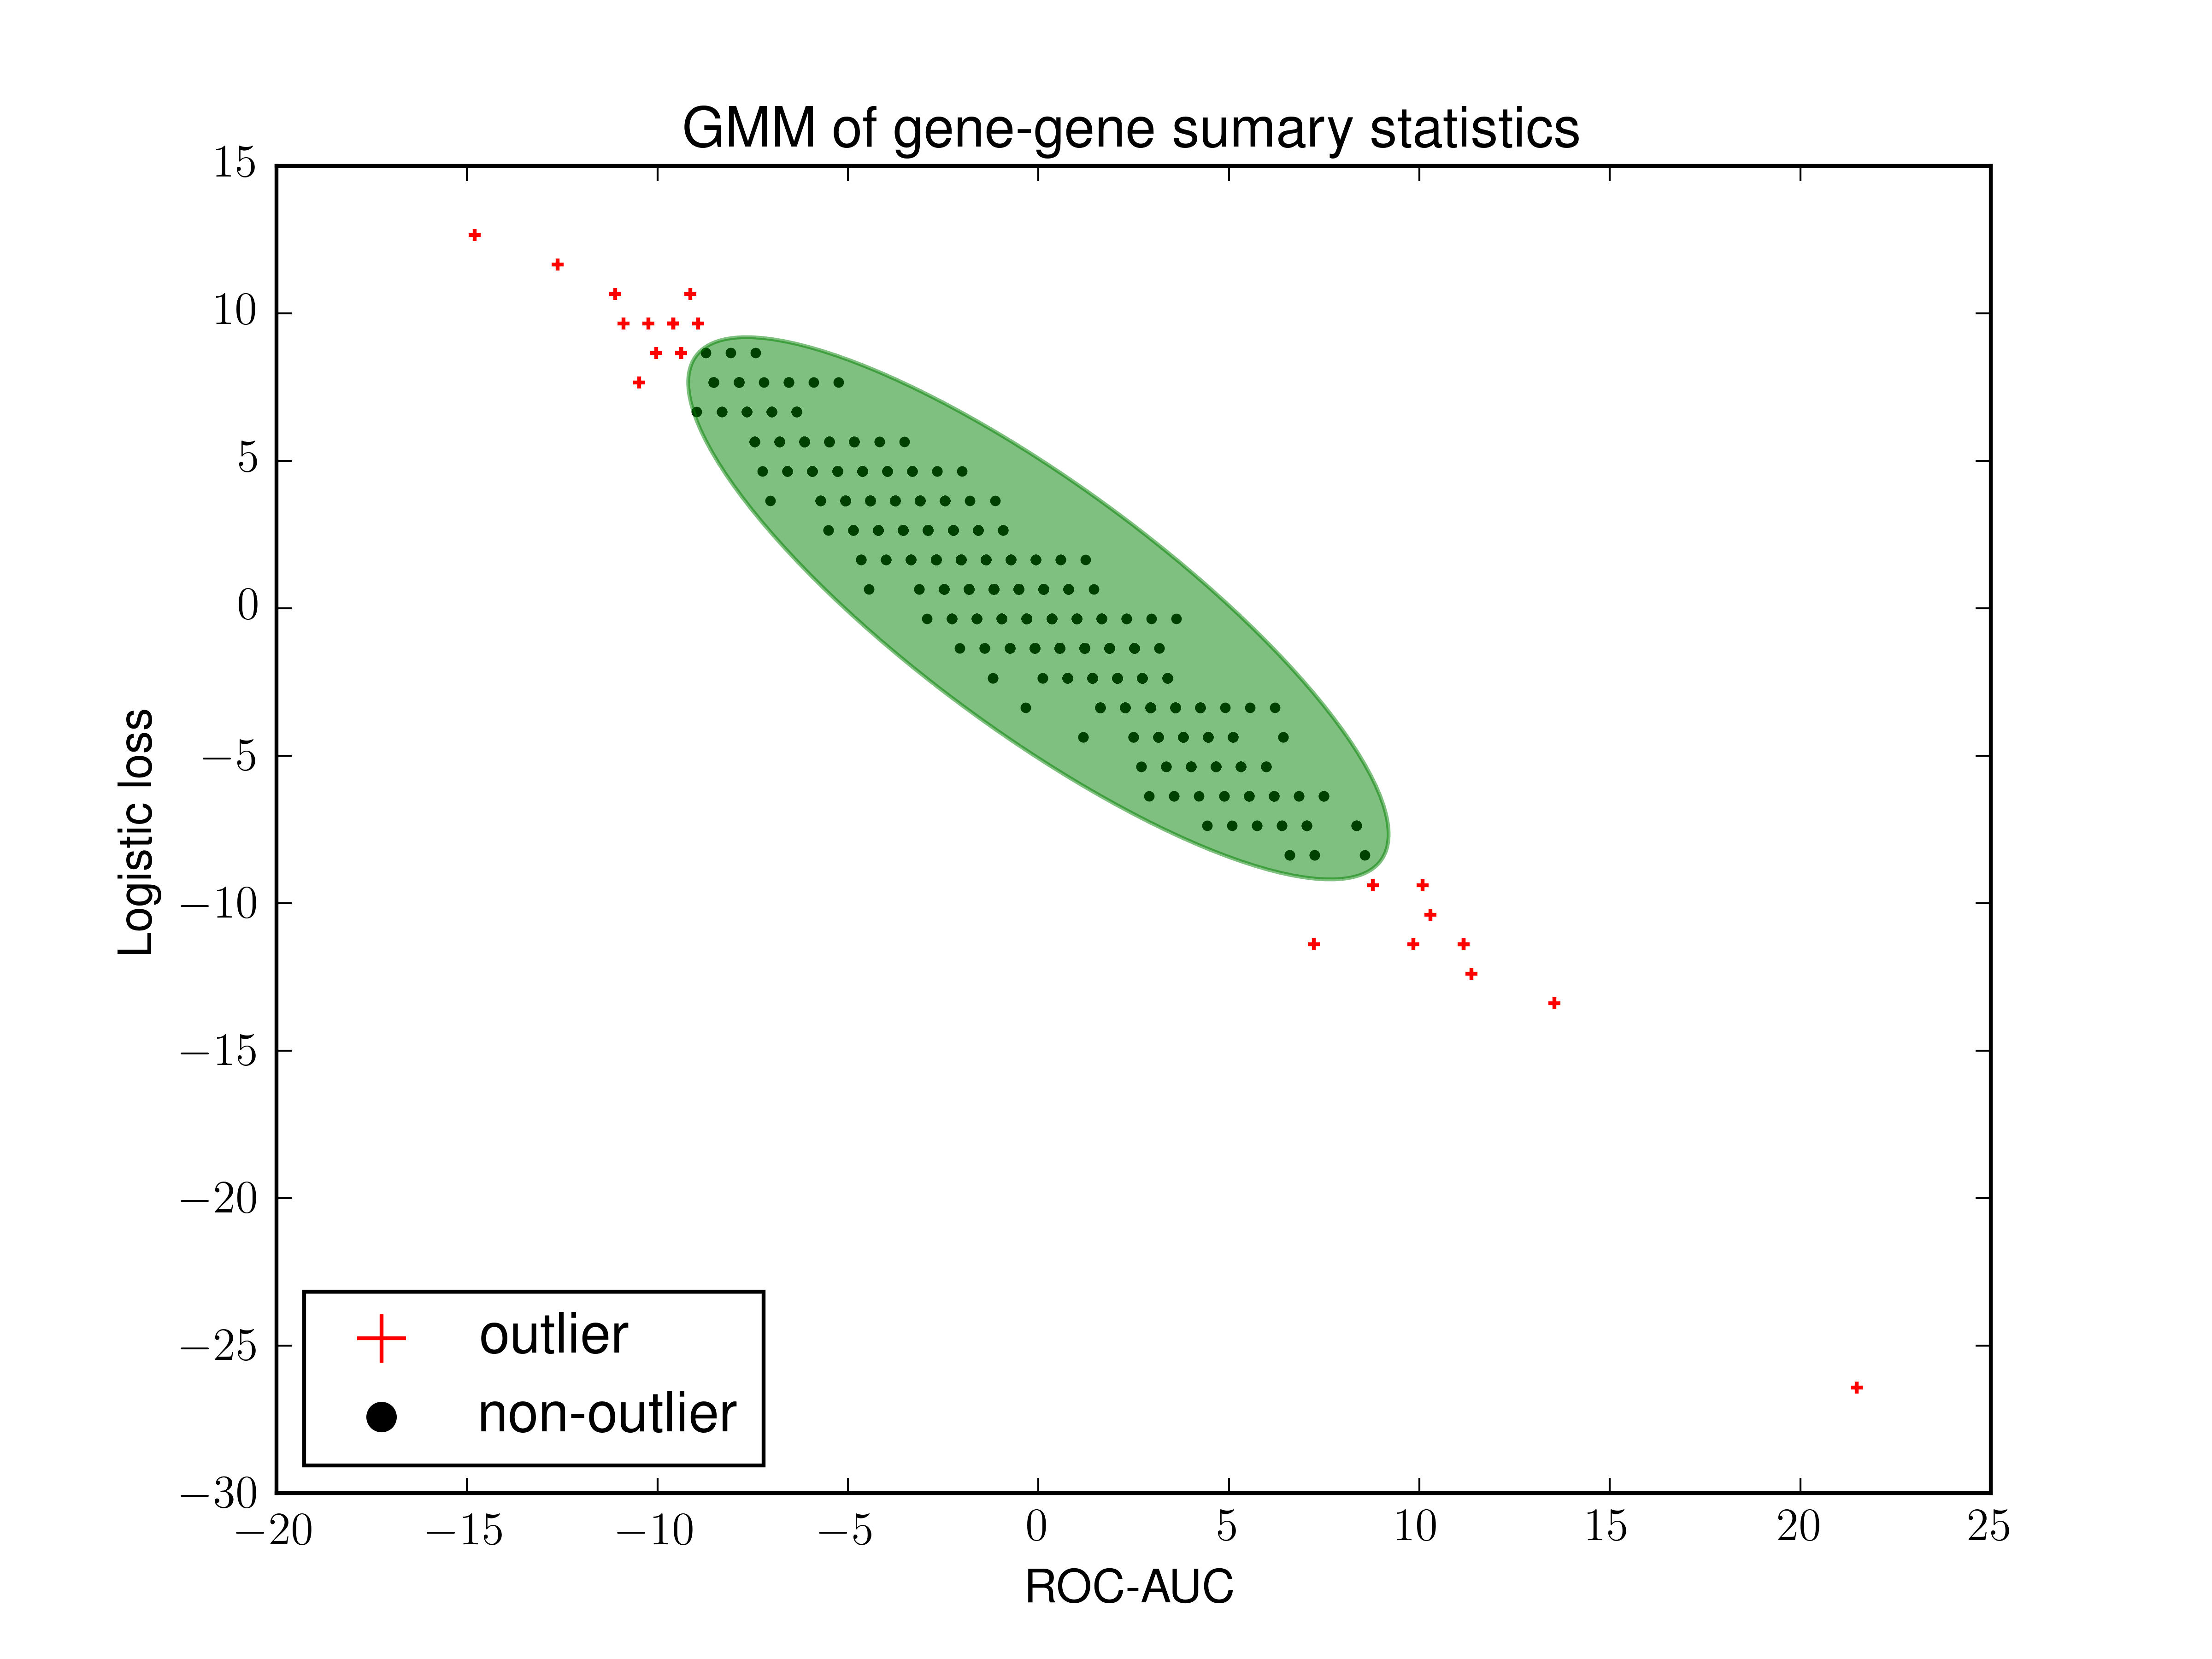
\includegraphics[width=6in]{./figs/gg-results-scatter.png}
            \end{center}
            \begin{flushleft}\small{\color{darkblue}Figure 5: \color{black} After running all pairwise combinations of variant-variant interactions summary statistics of predictive performance were plotted.  The two statistics: the area under the ROC curve and a logistic loss function are shown in standardized space.  A Gaussian mixture model (GMM) has been overlaid to determine outliers.}\end{flushleft}.
            \label{fig:application} 
            \end{figure} 
           }  
           
          \end{block}       
    \end{column}
    
    %%%%%%%%%%%%%%%%%%%%%%%%%%%%%%%%%%%%%%%%%%%%%%%%%%%%%%%%%%%%%%%%%%%%%%%%%%%%%%%%%%%%%%%%%%%%%%%%%%%%%%%%%%%%%
    % Fourth Column
    %%%%%%%%%%%%%%%%%%%%%%%%%%%%%%%%%%%%%%%%%%%%%%%%%%%%%%%%%%%%%%%%%%%%%%%%%%%%%%%%%%%%%%%%%%%%%%%%%%%%%%%%%%%%%
    \begin{column}{\sepwid}\end{column}
    \begin{column}{\onecolwid}
     \rmfamily{\scriptsize
	\begin{table}
	\begin{center}
       \begin{tabular}{|cc|cc|cc|}
       \hline
       Variant1  & Variant2 & Gene 1 & Gene 2 & $p$-value & $p$-value 2  \\
       \hline
       rs2074225   & rs4245191   & CD6       & NLRX1     & 1.21e-05 & 7.72e-06 \\
       rs9284879   & rs6120033   & TOPAZ1    & EFCAB8    & 5.96e-05 & 4.75e-05 \\
       rs3814355   & rs12976493  & CCNT2     & ADGRE2    & 1.46e-07 & 2.22e-16 \\
       snv3311     &rs1056286    & CELA1     & IL17RE    & 2.22e-16 & 0.0001 \\
       rs3814355   & snv469      & CCNT2     & LIMD1     & 1.46e-07 & 2.22e-16 \\
       snv469      & rs1136905   & LIMD1     & HLA-DRB5  & 2.22e-16 & 2.22e-16 \\
       rs11638215  & rs1136905   & SECISBP2L & HLA-DRB5  & 8.15e-05 & 2.22e-16 \\
       rs138579161 & snv2825     & RESP18    & BPIFC     & 2.22e-16 & 1.84e-07 \\
       rs3814355   & rs1136905   & CCNT2     & HLA-DRB5  & 1.46e-07 & 2.22e-16 \\
       rs147889095 & rs1136905   & ITPKB     & HLA-DRB5  & 1.25e-06 & 2.22e-16 \\
       snv1454     & rs10418767  & MUC6      & ADGRE2    & 2.07e-07 & 2.22e-16 \\
       rs1129152   & snv469      & INTS8     & LIMD1     & 0.0001   & 2.22e-16 \\
       snv3311     & rs9284879   & CELA1     & TOPAZ1    & 2.22e-16 &  5.98e-05 \\
       snv3311     & rs11638215  & CELA1     & SECISBP2L & 2.22e-16 &  8.15e-05 \\
       rs2308628   & rs12976493  & HLA-C     & ADGRE2   & 2.22e-16  & 2.22e-16 \\
       rs3814355   & rs11085765  & CCNT2     & MUC16    & 1.46e-07  & 1.73e-14 \\
       rs9284879   & snv1454     & TOPAZ1    & MUC6     & 5.98e-05  & 2.07e-07 \\
       snv2825     & rs192690014 & BPIFC     & HRNR     & 1.84e-07  & 2.22e-16 \\
       snv1454     & snv2825     & MUC6      & BPIFC    & 2.07e-07  & 1.84e-07 \\
       rs9284879   & rs1142888   & TOPAZ1    & GBP4     & 5.98e-05  & 6.04e-08 \\
       snv3311     & rs11085765  & CELA1     & MUC16    & 2.22e-16  & 1.74e-14 \\
       rs12976493  & snv469      & ADGRE2    & LIMD1    & 2.22e-16  & 2.22e-16 \\
       rs1056286   & rs10418767  & IL17RE    & ADGRE2   & 0.0001    & 2.22e-16 \\
       rs72268642  & rs6120033   & CNTNAP2 & EFCAB8    & 3.42e-07 & 4.75e-05 \\
       snv2825     & rs3814355   & BPIFC     & CCNT2    & 1.84e-07  & 1.46e-07 \\
       rs192690014 & rs3208105   & HRNR      & HLA-DQA1 &2.22e-16   & 2.22e-16 \\
       \hline
       \end{tabular}
       \end{center} 
       \begin{flushleft}\small{\color{darkblue}Table 2: \color{black} Gene-gene interactions prioritized by GMM log($p-$value)}\end{flushleft}.
           \label{fig:manhattan}
       \end{table}
       }  
     
    \begin{block}{Discussion}
          \rmfamily{
          The gene-gene interactions are based on a proxy of classification potential or more specifically how much that classification potential is perturbed when the pair of variants are removed from the analysis.  Both the significant genes from these analyses as well as the significant interactions appear to be relevant to disease.  Because these are preliminary results, both corroboration with the literature as well as independent experiments will help shed light on the reliability of these predictions.  It is also important that these methods be carefully contrasted with count-based methods for determining individual variant significance. 
          }
         \end{block}
        \begin{block}{References}
        \tiny
         \rmfamily{\begin{thebibliography}{99}
        \bibitem{Benjamini95} Y. Benjamini and Y. Hochberg, Controlling the False Discovery Rate: A Practical and Powerful Approach to Multiple Testing Journal of the Royal Statistical Society. Series B (Methodological), Blackwell Publishing for the Royal Statistical Society, 57, 289-300, 1995
        \bibitem{Li09} H. Li and R Durbin, Fast and accurate short read alignment with Burrows-Wheeler transform Bioinformatics, 25, 1754-60, 2009
        \bibitem{McKenna10} A. McKenna, M. Hanna \textit{et al}. The Genome Analysis Toolkit: a MapReduce framework for analyzing next-generation DNA sequencing data. Genome research, 20, 1297-303, 2010
        \bibitem{Seibold11} M. Seibold, A. Wise \textit{et al}.  A common MUC5B promoter polymorphism and pulmonary fibrosis N Engl J Med., 364, 1503-12, 2011
        \bibitem{Stuart15} B. D. Stuart, J Choi \textit{et al}. Exome sequencing links mutations in \textit{PARN} and \textit{RTEL1} with familial pulmonary fibrosis and telomere shortening Nature genetics, 47, 512-7, 2015
        \normalsize
        \end{thebibliography}}
        \end{block}        
        \begin{block}{Acknowledgements}
        \scriptsize 
        \rmfamily{Support for this work is provided by the NIH (R01 HL097163 and P01 HL092870) and the VA Merit Review Program (1I01BX001534).  Also, this work would not have been possible without the valuable contributions of several collaborating clinicians.  The opinions, findings and recommendations expressed in this work are those of the authors and do not necessarily reflect the views of the UC Denver or other affiliates.}
        \end{block}        
    \end{column}
    \begin{column}{\sepwid}\end{column}
\end{columns}
%\end{columns}
\end{frame}
\end{document}